\chapter{IoT Attacks and Safety implications}

\section{Growing IoT attacks}
Cyberattacks on IoT devices have increased greatly in the past years \cite{forbes}, and this trend will only continue in the future. This, coupled with the fact that almost half of businesses claim not to be able to detect IoT security breaches in their devices \cite{gemalto}, reveals the need for the improvement of IoT device protection from cyberattacks and detection of malicious behaviour.\\

\section{IoT Vulnerabilities}
Since IoT devices have applications in many different fields, each with varying energy and hardware constraints and with different communication methodologies, the attack surface for cybercriminals is very wide, and the design of IoT devices needs to carefully examine the potential vulnerabilities and the corresponding protections that need to be implemented.
    
To aid in the detection and prevention of attacks, and the development of security systems to protect IoT devices, multiple security principles have been identified by Staddon, E. et al \cite{IoT_categorization}, shown in Figure \ref{fig:security_principles} below, that need to be addressed in the design phase to achieve a secure design.\\

\begin{figure}[h]
    \centering
    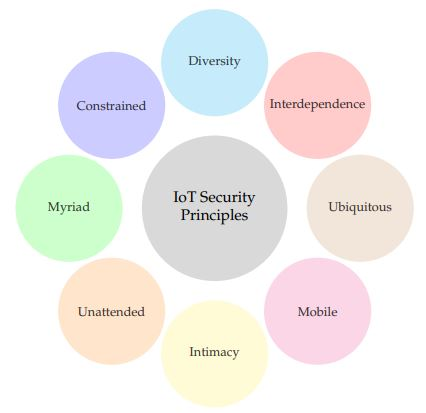
\includegraphics[width=.9\linewidth]{images/IoT security principles.JPG}
    \caption{IoT security principles proposed in the paper}
    \label{fig:security_principles}
\end{figure}

Take for example the Interdependence security principle,it states that since IoT systems are increasingly interconnected, the need for human interaction is diminished and allows for attackers to modify the system's behaviour by interfering with a single device. One real world use case would be a set of smart lightbulbs controlled by a light sensor, if the attackers gained control of the light sensor, they could send some malicious information to turn off the lightbulbs and irrupt into the house undetected.

Each of these security pillars need to be carefully studied when deploying an IoT solution, in order to help prevent attacks.


\section{Types of attacks on IoT devices}
Because of the nature of IoT devices, they are vulnerable to a wide array of attacks, in order to address the issue of classifying these attacks, Staddon, E. et al \cite{IoT_categorization} propose several categorization methods for IoT attacks, including labeling attacks based on the severity of the attack, the attack type or the access type, to name a few.\\

One of the proposals is to divide the attacks into three level related categories, \emph{Low-level}, \emph{Intermediate-level} and \emph{High-level} security issues. Low-level security issues encompasses threats to the lowest network layers, but also to the device's physical state. This includes attacks such as jamming, which disrupts network communication by saturating the communication channel or Denial of Sleep, in which the IoT device is constantly "kept awake" by issuing requests or by other means and this way the battery of the device is drained considerably more rapidly than it normally would, resulting in a DoS attack, another type of low-level attack is ARP-Spoofing, where a malicious attacker can access, modify or even stop data-in transit by obtaining a legitimate computer's IP address through malicious Address Resolution Protocol (ARP) messages.\\

Intermediate-level attacks are labeled as those directed against the network and all transport layer related activities, such as a routing and session management. Some examples of Intermediate-level attacks are Replay attacks, where data transmission is maliciously repeated or delayed, or a Sinkhole attack, where a malicious set of nodes modify the network traffic in order to prevent the base node from receiving the correct information.\\

The final High-level attacks are those that target the application themselves, they revolve around application vulnerabilities, such as insecure public interfaces, causing a breach to data privacy, or insecure software/firmware, allowing the attacker to take advantage of injection attacks like SQL or XML-injection.\\

It is important to highlight that this is just one of the dozens of categorization methods that exist for cyberattacks on IoT devices. From a security perspective it is interesting to study several categorization methods and offer protection against the types of attacks a specific IoT system might be vulnerable to.\\


\section{Safety and security implications of IoT attacks}
Since the attack surface on IoT devices is so big, many different severe consequences can result from a successful IoT cyberattack, we will look at some real world examples to understand the scale of the damage that could be inflicted.
\\~\\
One example would be the exploit of a \hyperlink{https://thehealthcareblog.com/blog/2019/07/29/security-crisis-of-cardiac-pacemakers-paves-the-way-for-iot-security-evolution-in-cardiology/}{vulnerability detected in 475k pacemakers}, this attack would expose critical health parameters of thousands of people that could be manipulated to cause harm/death.
\\~\\
Another IoT system in which attacks could have critical consequences is the smart-cars, which are rising in popularity, and \hyperlink{https://www.lifewire.com/how-self-driving-cars-can-be-hacked-5114337}{many possible attacks have already been proven to exist}, endangering not only the occupants of the car, but also other external actors. 
\\~\\
In general, we can observe that the IoT industry is vulnerable to many different types of attacks with very high damage potential, which is why protection, prevention and detection of these attacks is extremely necessary.


